% Algorithm Diagram
\begin{tikzpicture}[roundnode/.style={circle, draw=green!60, fill=green!5, very
thick, minimum size=7mm}, squarenode/.style={rectangle, draw=red!60, fill=red!5,
very thick, minimum size=5mm},
]
    \node[squarenode](start) {START};
    \node[roundnode](database) [right=of start] {\begin{tikzpicture}
    \draw[thin] (0,2) rectangle (3,4);
    \draw[thin] (0, 2.5) -- (3, 2.5);
    \draw[thin] (0, 3) -- (3, 3);
    \draw[thin] (0, 3.5) -- (3, 3.5);
    \draw[thin] (1, 2) -- (1, 4);
    \draw[thin] (2, 2) -- (2, 4);
    \node at (0.05, 4.25) {\footnotesize create database};
\end{tikzpicture}
};
    \node[squarenode](while) [right=of database] {WHILE NOT STOPPED};
    \node[roundnode](defector) [below=of database] {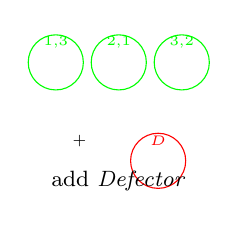
\begin{tikzpicture}
    \draw[green] (0.2, -1) circle (0.35);
    \node[green] at (0.2, -0.75) {\tiny 1,3};
    \draw[green] (1, -1) circle (0.35);
    \node[green] at (1, -0.75) {\tiny 2,1};
    \draw[green] (1.8, -1) circle (0.35);
    \node[green] at (1.8, -0.75) {\tiny 3,2};
    \node at (0.5, -2) {\tiny +};
    \draw[red] (1.5, -2.25) circle (0.35);
    \node[red] at (1.5, -2) {\tiny \(D\)};
    \node at (1, -2.5) {\footnotesize add \textit{Defector}};
\end{tikzpicture}};
    \node[roundnode](select_strat) [right=of defector] {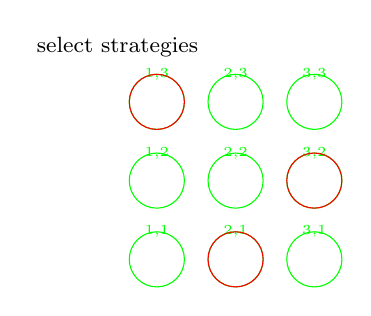
\begin{tikzpicture}
    %\draw[thin, dashed] (0, 0) rectangle (3, 3);
    \foreach \x in {1, 2, 3}
        \foreach \y in {1, 2, 3}
            {\draw[green] (\x-0.5, \y-0.5) circle (0.35);
            \node[green] at (\x-0.5, \y-0.15) {\tiny \x,\y};}
    \node at (0, 3.2) {\footnotesize select strategies};
    \draw[red] (1-0.5, 3-0.5) circle (0.35);
    \draw[red] (2-0.5, 1-0.5) circle (0.35);
    \draw[red] (3-0.5, 2-0.5) circle (0.35);
\end{tikzpicture}};
   \node[squarenode](noise&probs) [left=of defector] {FOR ALL $p_{n}$ \& $p_{e}$};
   \node[roundnode](payoffs) [below=of defector] {\begin{tikzpicture}
    \node at (-0.5, 0) {\tiny payoffs};
    \draw[->, thick] (0.5, 0) -- (0.75, 0);
    \draw[blue, dashed] (0.75, -0.25) rectangle (1, 0.25);
    \draw[blue] (1, -0.5) rectangle (2, 0.5);
    \draw[blue, dashed] (2, -0.25) rectangle (2.25, 0.25);
    \draw[->, thick] (2.25, 0) -- (2.5, 0);
    \node at (3.5, 0) {\tiny Nash eq.};
    \node at (0, 2) {\footnotesize calculating Nash eq.};
    %\node[above] at (1.75, -0.25) {\tiny support enumeration algorithm};
\end{tikzpicture}};
   \node[roundnode](tournament) [left=of payoffs] {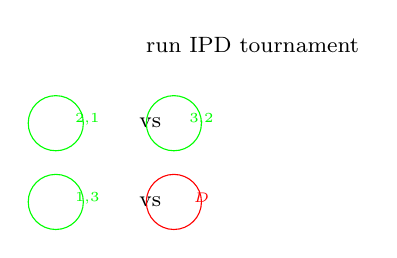
\begin{tikzpicture}
    \draw[green] (0,0) circle (0.35);
    \node[green] at (0.4, 0.05) {\tiny 2,1};
    \node[thick] at (1.2, 0) {\footnotesize vs};
    \draw[green] (1.5, 0) circle (0.35);
    \node[green] at (1.85, 0.05) {\tiny 3,2};
    \draw[green] (0, -1) circle (0.35);
    \node[green] at (0.4, -0.95) {\tiny 1,3};
    \node[thick] at (1.2, -1) {\footnotesize vs};
    \draw[red] (1.5, -1) circle (0.35);
    \node[red] at (1.85, -0.95) {\tiny \(D\)};
    \node at (2.5, 1) {\footnotesize run IPD tournament};
\end{tikzpicture}};
   \node[squarenode](writing) [right=of payoffs] {WRITE RESULTS TO DATABASE};
   \draw[->] (start.east) -- (database.west);
   \draw[->] (database.east) -- (while.west);
   \draw[->] (while.east) -- (15, 0) |- (select_strat.east);
   \draw[->] (select_strat.west) -- (defector.east);
   \draw[->] (defector.west) -- (noise&probs.east);
   \draw[->] (noise&probs.west) -- (-6, -6.12) |- (tournament.west);
   \draw[->] (tournament.east) -- (payoffs.west);
   \draw[->] (payoffs.east) -- (writing.west);
   \draw[->] (writing.east) -- (16, -13.1) |- (select_strat.east);
\end{tikzpicture}
